%%---------------------------------------------------------------------------%%
%% compile.tex
%% Time-stamp: <99/02/11 18:42:51 tme>
%% explains how to configure and compile the draco library
%%---------------------------------------------------------------------------%%

\chapter{Configuring and Compiling Draco}
\label{chap:compile}

This chapter describes how to configure and build \draco.  All
configure\index{configure} options will be illuminated in detail.  After reading this
chapter the user and/or developer will know how to build \draco\ on
multiple platforms, for various build project systems (\soft{Makefiles}, \soft{Eclipse}, \soft{XCode}, etc.) and for different options.  In addition, the user
will know how to build multiple versions of \draco\ simultaneously.
To illucidate the concepts about \draco\ dependencies, configuration
options, and build targets, \S~\ref{sec:examples} provides several
examples that show how to build \draco\ for various configurations.

%%---------------------------------------------------------------------------%%

\section{Draco Dependencies}
\label{sec:draco_dependencies}

As mentioned in \S~\ref{sec:overview_of_draco}, \draco\ is based on
the concept of levelized design~\cite{la96} \index{levelized design}.  A component-level diagram
is shown in Fig.~\ref{fig:level}\index{levelized design}.  By following the dependency lines
\begin{figure}
  \centerline{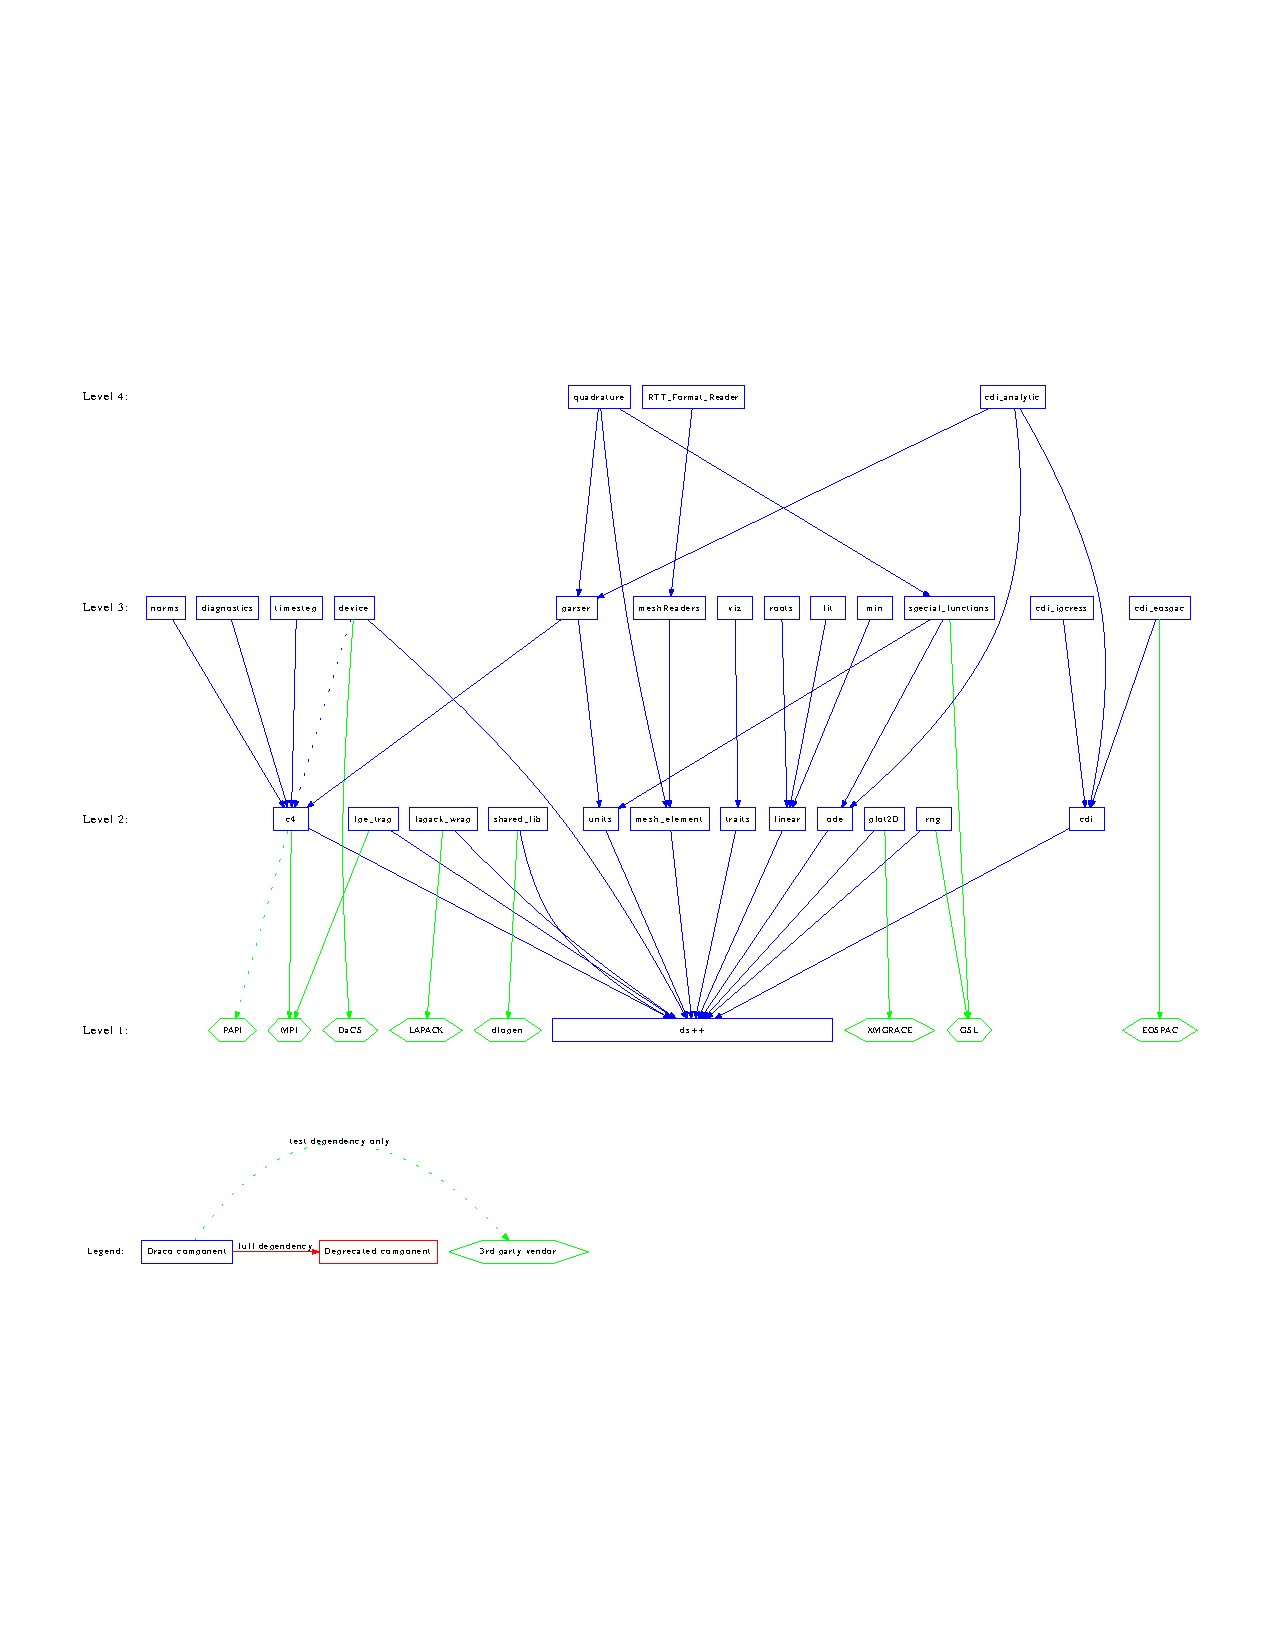
\includegraphics[angle=90]{fig/level}}
  \caption{Component-level diagram for \draco.}
  \label{fig:level}
\end{figure}
of this diagram, one can determine the exact dependencies required by
each component in \draco.  Thus, to compile a component static library, all of
the dependencies, both explicit and implicit, must be included when linking.

In addition to the direct component dependencies illustrated in
Fig.~\ref{fig:level}, the \comp{\vble{pkg}/test/} directory may
require additional components for its compartmentalized unit tests.  For example,
\comp{device} does not explicitly require \comp{c4}, but \comp{c4} and \comp{MPI} are required for compiling the unit tests for \comp{device}.  Unit test dependencies are included in this component-level diagram and dependencies unique to the tests are represented by dotted lines.   
%Figure~\ref{fig:test_level} shows the \draco\ package
%dependency tree
%\begin{figure}
%  \centerline{\includegraphics{fig/test_level.eps}}
%  \caption{Package-level diagram for \draco.  Test dependencies are
%    noted by the dotted arrows.}
%  \label{fig:test_level}
%\end{figure}
%with package test dependencies included.
The policy in \draco\ is that
test directories are responsible for their own template instantiations\index{policy!templates} in \comp{*\_pt.cc} files.
Directions showing how to include test directory dependencies are given in Chap~\ref{chap:adding}. 

When using \draco\ on an external product, all component dependent
libraries must be included.\index{dependencies!component}  The list of necessary libraries for
linking a package is given in Table~\ref{tab:depends}.  In summary,
\begin{table}
  \caption{
    Listing of \draco\ component dependencies.  The \draco\ component
    dependencies are the sum of the explicit and implicit dependencies.
    For general package use, only components listed under \draco\ Component
    Dependencies (Explicit and Implicit) are required.  The components
    listed under \draco\ Component Test Dependencies are only required for
    testing.}
  \label{tab:depends}
  \begin{center}
    \begin{tabular}{lclll} \hline\hline
      \multicolumn{1}{c}{\draco\ Package} & Level &
      \multicolumn{1}{c}{\draco\ Explicit} &
      \multicolumn{1}{c}{\draco\ Implicit} &
      \multicolumn{1}{c}{\draco\ Package} \\ 
      & & \multicolumn{1}{c}{Package Dependencies} &
      \multicolumn{1}{c}{Package Dependencies} &
      \multicolumn{1}{c}{Test Dependencies} \\ \hline
       \dsxx & 1 & - & - & - \\

%       \xm & 1 & - & - & - \\
%       \pkg{nml} & 2 & \dsxx & - & - \\
       \cfour & 2 & \dsxx & - & - \\
       \pkg{cdi} & 2 & \dsxx & - & - \\
       \pkg{fpe\_trap} & 2 & \dsxx & - & - \\
       \pkg{lapack\_wrap} & 2 & \dsxx & - & - \\
       \pkg{linear} & 2 & \dsxx & - & - \\
       \pkg{mesh\_element} & 2 & \dsxx & - & - \\
       \pkg{ode} & 2 & \dsxx & - & - \\
       \pkg{plot2D} & 2 & \dsxx & - & - \\
       \rng & 2 & \dsxx & - & - \\  
       \pkg{shared\_lib} & 2 & \dsxx & - & - \\
       \pkg{traits} & 2 & \dsxx & - & -  \\ 
       \pkg{units} & 2 & \dsxx & - & - \\       
       
%       \pkg{diffusion} & 3 & \pkg{nml} & \dsxx & \pkg{mesh} \\
%         \imc & 3 & \dsxx, \rng, \cfour & - & - \\
%       \pkg{linalg} & 3 & \dsxx, \cfour, \pkg{nml} & - & - \\
%       \pkg{mesh} & 3 & \dsxx, \pkg{xm}, \pkg{traits}, \cfour,
%       \pkg{nml} & - & - \\
%       \pkg{radphys} & 3 & \pkg{traits}, \pkg{units} & - &
%       \pkg{mesh} \\ 
       \pkg{cdi\_ipcress} & 3 & \pkg{cdi} & \dsxx & - \\
       \pkg{cdi\_eospac} & 3 & \pkg{cdi} & \dsxx & - \\
       \pkg{device} & 3 & \dsxx & - & \cfour \\
       \pkg{diagnostics} & 3 & \cfour & \dsxx & - \\
       \pkg{fit} & 3 & \pkg{linear} & \dsxx & - \\
       \pkg{meshReaders} & 3 & \pkg{mesh\_element} & \dsxx & - \\
       \pkg{min} & 3 & \pkg{linear} & \dsxx & - \\
       \pkg{norms} & 3 & \cfour & \dsxx & - \\
       \pkg{parser} & 3 & \cfour, \pkg{units} & \dsxx & - \\
       \pkg{roots} & 3 & \pkg{linear} & \dsxx & - \\
       \pkg{special\_functions} & 3 & \pkg{ode}, \pkg{units} & \dsxx & - \\
       \pkg{timestep} & 3 & \cfour & \dsxx & - \\
       \pkg{viz} & 3 & \pkg{traits} & \dsxx & - \\
       
       \pkg{cdi\_analytic} & 4 & \pkg{parser}, \pkg{ode}, \pkg{cdi} & \cfour, \dsxx, \pkg{units} & - \\
       \pkg{quadrature} & 4 & \pkg{parser},  & \cfour, \dsxx, \pkg{units},  & - \\
        &  & \pkg{mesh\_element},  & \pkg{ode} &  \\
        &  & \pkg{special\_functions} &  &  \\
              
%       \pkg{matprops} & 4 & \dsxx, \pkg{traits}, \pkg{units},
%       \pkg{radphys} & - & \pkg{mesh} \\
%       \pone & 4 & \dsxx, \pkg{linalg}, \pkg{diffusion} & \cfour,
%       \pkg{nml} & \pkg{mesh} \\ 
\hline\hline
    \end{tabular}
  \end{center}
\end{table}
when a \draco\ component is used in an external code, all libraries
listed under \draco\ Package Dependencies (Explicit and Implicit) in
Table~\ref{tab:depends} must be included on the link line.  The
packages listed under \draco\ Package Test Dependencies do not have to
be linked.  We note that \draco\ packages know both their package
dependencies and their package test
dependencies (Fig.~\ref{fig:level}).  The external \draco\ client
must be aware that when using a \draco\ package all of the packages
dependencies (not package test dependencies) must be included.

Some components in \draco\ require external vendor support.\index{dependencies!vendor}
Additionally, some configuration options in \draco\ require external
vendor support.  Table~\ref{tab:vendor} lists all of the present
\begin{table}
  \caption{Vendors required by packages in \draco.  Implicit are the
    \cpp\ Standard Template Library (STL), the \cc\ Standard
    Library, and compiler libraries (\comp{libF77}).  Systems
    libraries  (\comp{sys/time.h}) are also not included.}
  \label{tab:vendor}
  \begin{center}
    \begin{tabular}{lclc}\hline\hline
      \multicolumn{1}{c}{Package} & Level & \multicolumn{1}{c}{Vendor Options}
      & Required \\ \hline
      \dsxx & 1 & - &  - \\
      
%      \xm & 1 & - & - \\
      \cfour & 2 & \mpi, \sys{OpenMP} & no \\
      & & \sys{PAPI} & no \\
      \pkg{cdi} & 2 & - & - \\
      \pkg{fpe\_trap} & 2 & \mpi & no \\
      \pkg{lapack\_wrap} & 2 & \sys{LAPACK}, \sys{BLAS} & yes \\
      \pkg{linear} & 2 & - & - \\
      \pkg{mesh\_element} & 2 & - & - \\
      \pkg{ode} & 2 & - & - \\
      \pkg{plot2D} & 2 & \sys{XM Grace} & yes \\
      \pkg{rng} & 2 & \sys{GSL} & yes \\
      \pkg{shared\_lib} & 2 & \sys{dlopen} & yes \\
      \pkg{traits} & 2 & - & - \\
      \pkg{units} & 2 & - & - \\
      
%      \pkg{nml} & 2 & - & - \\
%      \rng & 2 & \sprng & yes  \\
%      \pkg{units} & 2 & - & - \\
%      \pkg{diffusion} & 3 & - & - \\
%      \imc & 3 & - & -  \\
%      \pkg{linalg} & 3 & \pcglib & yes \\
%      \pkg{mesh} & 3 & - & - \\
    %  \pkg{radphys} & 3 & - & - \\ 
          \pkg{cdi\_eospac} & 3 & \sys{EOSPAC} & yes \\
      \pkg{cdi\_ipcress} & 3 & - & - \\
      \pkg{device} & 3 & \sys{DaCS} or \sys{CUDA} & yes \\
       &  & \sys{MPI} & no \\
      \pkg{diagnostics} & 3 & \sys{MPI} & no \\
      \pkg{fit} & 3 & - & - \\
      \pkg{meshReaders} & 3 & - & - \\
      \pkg{min} & 3 & - & - \\
      \pkg{norms} & 3 & \sys{MPI} & no \\
      \pkg{parser} & 3 & \sys{MPI} & no \\
      \pkg{roots} & 3 & - & - \\
      \pkg{special\_functions} & 3 & \sys{GSL} & yes \\      
      \pkg{timestep} & 3 & \sys{MPI} & no \\
      \pkg{viz} & 3 & - & - \\
       
%      \pkg{matprops} & 4 & - & - \\
%      \pone & 4 & - & - \\ 
      \pkg{cdi\_analytic} & 4 & \sys{MPI} & no \\
      \pkg{quadrature} & 4 & \sys{GSL} & yes \\
       &  & \sys{MPI} & no \\
      \pkg{RTT\_Format\_Reader} & 4 & - & - \\

\hline\hline
    \end{tabular}
  \end{center}
\end{table}
components in \draco\ and the vendors that are required to build those
components.  Also, because \draco\ is based on the concepts of levelized
design as stated above, each component in \draco\ may have dependencies
on lower level \draco\ components.  In these cases only the dependencies
of the specified package are of interest.  For example, the \pkg{parser} 
component itself requires no external vendors; however, \pkg{parser} requires
\cfour\ that does require an external vendors (\sys{MPI}).  The build system
knows the \draco\ dependencies of each component; however, the external
user (client) must be aware of vendor requirements in the component
dependencies.  If a required vendor library is not found by the \draco\ build system, that component will be omitted from the configuration.  For example, if \sys{LAPACK} is not found on the current machine, the \draco\ build system will not attempt to configure or compile \pkg{lapack\_wrap}.  Some dependencies, like \sys{PAPI} are only used for profiling and if activated anywhere, must be activated everywhere.
Tables~\ref{tab:depends} and \ref{tab:vendor} can be
used to determine what \draco\ components and what vendor libraries must
be included when linking to a specific \draco\ components.  Details on
how to configure components with certain vendor options are given in
\S~\ref{sec:configuration_options}.  Information on linking to
specific libraries is given in Appendix~\ref{app:vendor_libs}.

To summarize the preceding we will employ a simple example.  Let us
assume that a user wishes to use the \pkg{quadrature} package.  Additionally,
this configuration will be a parallel configuration using
\mpi\,\footnote{\cfour\ is \draco's communication package and
  determines if the resulting code will be scalar or parallel.}.  From
Table~\ref{tab:depends} we see that \pkg{quadrature} is dependent on the \draco\ 
packages \pkg{special\_functions}, \pkg{parser}, \pkg{mesh\_element}, \pkg{ode}, \dsxx, \pkg{units}, and \cfour.  From Table~\ref{tab:vendor} we see
that \pkg{ode} requires the \sys{GSL} library and \cfour\ requires the \mpi\ 
library.  Accordingly, for a \sys{UNIX} \sys{Makefile}-based build, the following libraries must be included on the
link line:
\begin{verbatim}
     -lrtt_quadrature -lrtt_parser -lrtt_special_functions -lrtt_c4 -lrtt_units \
     -lrtt_mesh_element -lrtt_ode -lrtt_ds++ \
     -lgsl -lgslcblas \
     -lmpi_cxx -lmpi -lopen-rte -lopen-pal
\end{verbatim}
where \comp{-lgsl -lgslcblas} are the \pkg{GSL} libraries (see \S~\ref{appsec:gsl}) and \comp{-lmpi\_cxx -lmpi -lopen-rte -lopen-pal} are the \mpi\ libraries (see \S~\ref{appsec:mpi}).  Additional system libraries may also be required (e.g.: \comp{-ldl -lnsl -lutil -lm}).
This example assumes that all of the following library locations are
defined in \ldlib.  Thus, even though \pkg{quadrature} does not explicitly depend
on \mpi\ or \sys{GSL}, it uses \draco\ packages (\cfour\ and \pkg{special\_functions}) that
do require these libraries.  In practice, the \draco\ build system attempts to find and use full paths to vendor and \draco\ component libraries so that \ldlib\ does not need to be manipulated by the developer or software user.  The build system also locates and sets all of the libraries required or each vendor so that a \draco\ component or client only needs to specify that it should link to a set of libraries provided by the \cmake\ variable  \$\vble{\{\$\{VENDOR\}}\comp{\_LIBRARIES\}}.

%%---------------------------------------------------------------------------%%

\section{Draco Package Products}

In Chap.~\ref{chap:model} we insinuated that each \draco\ component
provides a library.  For example, \pkg{quadrature} provides
\comp{librtt\_quadrature.a(.so)} on \sys{UNIX} systems.  This is not entirely accurate.  Some \draco\
packages, \pkg{traits} is an example, consist only of header files and do not
provide a compiled library.  Users need to be aware of this fact when
linking \draco\ components.  If a \draco\ client uses the \pkg{viz}
package, which requires \pkg{traits}, linking \comp{-lrtt\_traits} is incorrect because
\pkg{traits} does not produce a library.  Table~\ref{tab:products} lists the
\begin{table}
  \caption{Products for \draco\ packages.}
  \label{tab:products}
  \begin{center}
    \begin{tabular}{lccc}\hline\hline
      \multicolumn{1}{c}{Package} & \comp{include/} & \comp{lib/} &
      \comp{bin/} \\ \hline
      
      \dsxx & yes & yes &  no \\
      
      \cfour & yes & yes & no \\
      \pkg{cdi} & yes & yes & no \\
      \pkg{fpe\_trap} & yes & yes & no \\
      \pkg{lapack\_wrap} & yes & no & no \\
      \pkg{linear} & yes & yes & no \\
      \pkg{mesh\_element} & yes & yes & no \\
      \pkg{ode} & yes & yes & no \\
      \pkg{plot2D} & yes & yes & no \\
      \pkg{rng} & yes & yes & no \\
      \pkg{shared\_lib} & yes & yes & no \\
      \pkg{traits} & yes & no & no \\
      \pkg{units} & yes & yes & no \\
      
      
      
      \pkg{cdi\_eospac} & yes & yes & no \\
      \pkg{cdi\_ipcress} & yes & yes & yes \\
      \pkg{device} & yes & yes & no \\
      \pkg{diagnostics} & yes & yes & no \\
      \pkg{fit} & yes & yes & no \\
      \pkg{meshReaders} & yes & yes & no \\
      \pkg{min} & yes & yes & no \\
      \pkg{norms} & yes & yes & no \\
      \pkg{parser} & yes & yes & no \\
      \pkg{roots} & yes & yes & no \\
      \pkg{special\_functions} & yes & yes & no \\
      \pkg{timestep} & yes & yes & no \\
      \pkg{viz} & yes & yes & no \\
                 
      \pkg{cdi\_analytic} & yes & yes & no \\
      \pkg{quadrature} & yes & yes & no \\
      \pkg{RTT\_Format\_Reader} & yes & yes & no \\
      
      \hline\hline
%      \multicolumn{4}{l}{$^{\text a}$\pkg{nml} uses a \perl\ script
%        \comp{nmlgen*} that} \\
%      \multicolumn{4}{l}{is installed in the \comp{libexec/}
%        directory.} \\
    \end{tabular}    
  \end{center}
\end{table}
\draco\ packages and their products.  Users must only link against
those products that make a library.  Note also that package executables
produced under the \vble{pkg}\comp{/test/} directories are not
considered executable products.

%%---------------------------------------------------------------------------%%

\section{Configuring Draco}
\label{sec:configuring_draco}

We have previously mentioned that building \draco\ is a two-step
process.  First, \draco\ must be configured for a particular build configuration and build tool.\index{configuring}
Second, \draco\ is built using particular build targets.  In this
section we shall concentrate on configuring \draco.  Note that many
details about \cmake\ and the \draco\ \cmake\ macros are glossed over in this
treatment.  Interested readers are referred to Ref.~\cite{cmake}
for more information.  Examples that illustrate the concepts described 
in this section are given in \S~\ref{sec:examples}.

\subsection{Preparing the target and binary directories}
\label{sec:running_configure_prepare}

Running \cmake\ is straightforward; however, setting up the target
directories where various builds will take place require some
consideration.  In \S~\ref{sec:draco_src_tree} we described how the
source tree is not necessarily where the build takes place.  In fact,
we advise that builds be performed in a location separate from the
source tree\footnote{The exception to this advice is when the target build tool is \sys{Eclipse CDT} where there are advantages to using a {\it within-source-tree build}, namely, better support for \svn\ through the \sys{Eclipse} IDE.}.  Through this method multiple builds (debug, optimized) can be performed
simultaneously using the same source files.  Additionally, the source tree will not be cluttered
by build-file remnants such as object dependency files.\index{build!within-source-tree}\index{build!out-of-source-tree}

Before running \cmake\ to configure your build directory, we set up target and binary directory trees\index{directory!binary}\index{directory!target}.  Note
that this directory can be the same as the source directory; although,
we do not recommend this strategy.  The target directory name should
be descriptive of the particular build that is being performed.  For
example to build a debug version on a Linux platform with \mpi\ support, one might make
a directory entitled \comp{linux\_\,mpid/}. Thus, for \sys{Unix} systems the user enters
\begin{verbatim}
     $ mkdir -p linux_mpid/draco
\end{verbatim} % $
Similar directory creation processes should be used on other platforms.  Note that we do not require a \comp{draco/} binary directory under the target
directory.  However, this strategy does alleviate the complexity when
using \draco\ with other code systems.  If the user is planning on
using a product that emulates the \draco\ build system, such as
\capsaicin, \clubimc\  or \milagro, then parallel binary directories should be
added for each product
\begin{verbatim}
     $ cd linux_mpid
     $ mkdir capsaicin
     $ mkdir clubimc
     $ mkdir milagro
\end{verbatim}
Details on using the \draco\ build model in external products are
reserved until Chap.~\ref{chap:extern}.

\subsection{Running CMake from the command line}
\label{sec:running_configure_cmd_line}

The next step is to run the \cmake\ command line tool inside the \draco\ binary directory.  If you prefer, you can run the interactive \cmake\ tools described in \S~\ref{sec:running_configure_ccmake} and \S~\ref{sec:running_configure_cmakegui}.  We assume that the \draco\ source tree lives at \dracohome.  
To generate a build project in the binary dreictory, run \cmake\ from the \draco\ binary directory, \comp{linux\_\,mpid/draco/} and provide the location of the \draco\ source tree as a \cmake\ argument.  Most importantly, we need to set the
install directory\index{directory!install}, denoted by \comp{CMAKE\_INSTALL\_PREFIX} on the \cmake\ command line\footnote{This can also be set in the file \comp{linux\_\,mpid/draco/CMakeCache.txt}, or in the GUI interface provided by \comp{ccmake} or \comp{cmake-gui}.}.  To set a build parameter on the \cmake\ command line we use the \cmake\ option \comp{-D}.  An example \cmake\ configuration command for a \sys{UNIX} \sys{Makefile} configuration is illustrated here:
\begin{verbatim}
      $ cd linux_mpid/draco
      $ cmake -DCMAKE_INSTALL_PREFIX=.. $draco_home
\end{verbatim}
The first option sets the install location to the target directory, \comp{linux\_\,mpid/}.  The second option provides the source location of \draco\ and the controlling \comp{CMakeLists.txt} file.
%This may be accomplished in two ways.  One, the
%user may run the \dracoconf\ script that comes with the \draco\ 
%distribution.  This script requires the user to set the
%\comp{--prefix} directory as an argument to the script. The following
%examples illustrate this option:
%\begin{verbatim}
%     $ cd sgi_mpi/draco
%     $ $draco_home/draco_config ..
%     $ $draco_home/draco_config .
%     $ $draco_home/draco_config /usr/local/contrib/draco
%\end{verbatim} % $
%The first option sets the install location in \comp{sgi\_\,mpi/}.  The
%second option sets the install location in \comp{sgi\_\,mpi/draco/}.
%The final option installs in \comp{/usr/local/contrib/draco/}.  The
%\dracoconf\ script will give an error if a \comp{--prefix} directory
%is not given.  
Note that additional options for \cmake\ are simply
appended to the command-line ahead of the source location.  Thus, to force the creation of static libraries for the \draco\ build,
we would enter
\begin{verbatim}
     $ cmake  -DCMAKE_INSTALL_PREFIX=.. -DDRACO_LIBRARY_TYPE=STATIC $draco_home
\end{verbatim}
More details on the configuration options are given in
\S~\ref{sec:configuration_options}.

%The second way to run configure is to manually run the
%\dracohome\comp{/configure*} script.  Thus, to repeat the options from 
%the preceding paragraph, the user must enter
%\begin{verbatim}
%     $ cd sgi_mpi/draco
%     $ $draco_home/configure --prefix=$home/sgi_mpi
%     $ $draco_home/configure --prefix=$home/sgi_mpi/draco
%     $ $draco_home/configure --prefix=/usr/local/contrib/draco
%\end{verbatim} % $
%where we have assumed that \comp{sgi\_\,mpi/} lives in \comp{\$home}.
%The differences between running \dracoconf\ and
%\dracohome\comp{/configure*} should now be apparent.  Configure
%expects the directory specified by \comp{--prefix} to be an absolute
%path.  \dracoconf\ allows the user to enter relative paths, and it
%converts these to absolute paths for configure.  Proceeding with our
%analysis, if the user wants to install \draco\ products in
%\comp{\$home/sgi\_\,mpi/} with \mpi\ then the following is required
%\begin{verbatim}
%     $ $draco_home/configure --prefix=$home/sgi_mpi --with-c4=mpi
%\end{verbatim} % $
%Additional configuration options are detailed in
%\S~\ref{sec:configuration_options}. 

Running \cmake\ in the \comp{draco/} binary directory within the target
directory (\comp{linux\_\,mpid/}) produces a directory tree under
the \comp{draco/} subdirectory that is parallel to the \draco\ source
directory tree.  This directory structure is illustrated in
Fig.~\ref{fig:build_tree}.  Note that we could have run \cmake\ 
under the target top-level directory (\comp{linux\_\,mpid/}).  If we had
proceeded with this strategy the contents of the \comp{draco/} target
subdirectory would be moved up one level.

One final point should be mentioned about \comp{CMAKE\_INSTALL\_PREFIX}.  \cmake's
default location for the installation directory is
\comp{/usr/local/} on \sys{UNIX} and \comp{\%ProgramFiles\%} on \sys{Windows}, but the build system will modify this value to point to an \comp{install} subdirectory located beneath the \draco\ binary diretory (e.g.: \comp{linux\_\,mpid/draco/install}) if the developer does not provide another location.  Thus, the user must enter a value for \comp{CMAKE\_INSTALL\_PREFIX} either on the command line or via the \cmake\ GUI 
explicitly to override the default.  The suggested method is to set
\comp{CMAKE\_INSTALL\_PREFIX} to the target directory (\comp{linux\_\,mpid/} in this
example).  This will allow multiple targets to be built simultaneously 
without risk of name collisions.

If the build configuration requires many options, the developer may choose to create a \comp{CMakeCache.txt} file\index{CMakeCache.txt} in the \draco\ binary directory before running \cmake\ for the first time.  All build options can set in the \comp{CMakeCache.txt} file so that the configuration command only requires the location of the sources:
\begin{verbatim}
    $ cd linux_mpid/draco
    $ ls
    CMakeCache.txt
    $ cmake $draco_home
\end{verbatim}
A sample \comp{CMakeCache.txt} file is provided in the root \draco\ source directory.  The contents of this file are also provided in Listing~\ref{lst:cmakecachetxt}.
%
\lstset{language=ksh,
  showstringspaces=false,
  frame=shadowbox,
  basicstyle=\footnotesize,
  rulesepcolor=\color{black},
  backgroundcolor=\color{listingBG}
}
\begin{lstlisting}[basicstyle=\footnotesize, xleftmargin=0.0in, xrightmargin=0.0in, caption={A sample \comp{CMakeCache.txt} file.}, float=tn,label={lst:cmakecachetxt}]
# CMakeCache.txt template for Draco
# $Id$

# Instructions.
# 1. Copy this file to your build directory as CMakeCache.txt.
# 2. Review and update all values in this file.
# 3. From the build directory run 'cmake /full/path/to/source'
# 4. make
# 5. ctest
# 6. make install

# ------------------------------------------------------------
# You must set these values for your build:
# ------------------------------------------------------------

# Location where 'make install' will copy files to.
# CMAKE_INSTALL_PREFIX:PATH=c:/Release-x64/draco
CMAKE_INSTALL_PREFIX:PATH=/var/tmp/kgt/cmake/gcc/mpid/t

# VENDOR_DIR:PATH=$ENV{VENDOR_DIR}
# Windows: k:/vendors/x64-Windows
VENDOR_DIR:PATH=/ccs/codes/radtran/vendors/Linux64

# CMAKE_BUILD_TYPE == { Release, Debug, RelWithDebInfo, MinSizeRel }
CMAKE_BUILD_TYPE:STRING=Debug

# CMAKE_GENERATOR == { NMake Makefiles, Unix Makefiles, 
#                      Visual Studio 9 2008, Visual Studio 9 2008 Win64 }
CMAKE_GENERATOR:STRING=Unix Makefiles

# ------------------------------------------------------------
# Review these additional settings
# ------------------------------------------------------------

# Should we compile the tests?
BUILD_TESTING:BOOL=ON

# C4 communication mode (SCALAR or MPI)
DRACO_C4:STRING=MPI

# Design-by-Contract (0-7)?
DRACO_DBC_LEVEL:STRING=7
 
# Keyword for creating new libraries (STATIC or SHARED).
DRACO_LIBRARY_TYPE:STRING=SHARED
\end{lstlisting} \index{CMakeCache.txt} \index{generator}
Developers can copy this file to the \draco\ binary directory and modify, comment out or add options as needed before running \cmake\ for the first time.

One final note about running \cmake\ from the command line is the option to choose a project {\it Generator}\index{generator}\index{cmake!generator}.  On \sys{UNIX} systems, the default generator is \sys{Unix Makefiles}, but \sys{Eclipse CDT4 - Unix Makefiles} is also supported.  To select an alternative generator, use the \comp{-G} command line argument for \cmake.  The full list of available generators can be obtained by running \comp{'cmake --help'}.

%% ---------------------------------------------------------------------------- %%
\subsection{Running CMake interactively from the command line}
\label{sec:running_configure_ccmake}

\cmake\ can be run in an interactive environment by running \comp{ccmake} from command line\index{ccmake}.  This configuration mode is similar to the the method described above in \S~\ref{sec:running_configure_cmd_line}.  To start the interactive configure session, navigate to the binary directory and run \comp{ccmake}
\begin{verbatim}
     $ cd linux_mpid/draco
     $ ccmake $draco_home
\end{verbatim}
This will start an interactive configure session that will look similar the screenshot shown in Listing~\ref{lst:ccmake-empty}.
\begin{lstlisting}[basicstyle=\footnotesize, xleftmargin=0.0in, xrightmargin=0.0in, caption={The \comp{ccmake} screen prior to running configure.}, float=htn, label={lst:ccmake-empty}]
                                                     Page 0 of 1
 EMPTY CACHE


EMPTY CACHE:                                                                              
Press [enter] to edit option                                       CMake Version 2.8.8-rc1
Press [c] to configure
Press [h] for help           Press [q] to quit without generating
Press [t] to toggle advanced mode (Currently Off)
\end{lstlisting}
Selecting interactive command \comp{[c]} (followed by \comp{[e]} to exit the output review screen) 
will populate the configure environment with default values (be sure to turn caps lock off) resulting in something similar to what is shown in Listing~\ref{lst:ccmake-post-configure}.
\begin{lstlisting}[basicstyle=\footnotesize, xleftmargin=0.0in, xrightmargin=0.0in, caption={The \comp{ccmake} screen after the initial configure command.}, float=htn, label={lst:ccmake-post-configure}]
                                                     Page 1 of 1
 BUILD_AUTODOC                   *OFF                                                    
 BUILD_DOC                       *OFF                                                    
 BUILD_TESTING                   *ON                                                     
 BUILD_USE_SOLUTION_FOLDERS      *ON                                                     
 CMAKE_BUILD_TYPE                *Debug                                                  
 CMAKE_INSTALL_PREFIX            */var/tmp/gcc-mpid/d/install                        
 DRACO_C4                        *MPI                                                    
 DRACO_DBC_LEVEL                 *7                                                      
 DRACO_DIAGNOSTICS               *0                                                      
 DRACO_LIBRARY_TYPE              *SHARED                                                 
 DRACO_TIMING                    *0                                                      
 DRACO_VERSION                   *6.3                                                    
 DRACO_VERSION_FULL              *6.3.20120412                                           
 ENABLE_RNG_NR                   *OFF                                                    
 GCC_ENABLE_ALL_WARNINGS         *OFF                                                    
 GCC_ENABLE_GLIBCXX_DEBUG        *OFF                                                    
 GSL_FOUND                       *ON                                                     
 NUMDIFF                         */ccs/codes/radtran/vendors/numdiff-5.2.1/bin/numdiff   
 USE_OPENMP                      *ON                                                     
 VENDOR_DIR                      *              

BUILD_AUTODOC: OFF                                                                                                                                                         
Press [enter] to edit option                                       CMake Version 2.8.8-rc1
Press [c] to configure
Press [h] for help           Press [q] to quit without generating
Press [t] to toggle advanced mode (Currently Off)
\end{lstlisting}
To modify the target location navigate to the \comp{CMAKE\_INSTALL\_PREFIX} line and press enter to edit the path location.  \comp{ccmake} navigation and editing commands can
be found by selecting the \comp{[h]} option.  Similarly, the build can be configured to generate static libraries by editing the \comp{DRACO\_LIBRARY\_TYPE} value and setting it to \comp{STATIC}.  Once the build settings are complete, select the \comp{[c]} (configure) option two more times to complete the configuration process and review the new values.    To generate the controlling build project files (e.g.: \sys{Makefiles}), select the \comp{[g]} (generate) option.  The most common build features are shown in the default \comp{ccmake} environment.  In some cases, the developer may need to edit an {\it advanced} build variable.  The list of all variables can be viewed by the \comp{[t]} (toggle) advanced values option.

%% ---------------------------------------------------------------------------- %%
\subsection{Running CMake interactively through the GUI}
\label{sec:running_configure_cmakegui}

\cmake\ can be run in an interactive graphical user interface (GUI) by running \comp{cmake-gui} either from the command line for by selecting the tool from the operating system's toolbar (this tool may not be available for all systems).\index{cmake-gui}  This configuration mode is similar to the the methods described above in \S~\ref{sec:running_configure_cmd_line}-\ref{sec:running_configure_ccmake}.  This tool can be started from any directory because the source and binary locations must always be provided manually, when using the GUI tool.  As in the previous section, after providing the source and binary directory locations, select the {\it Configure} button to populate the Cache with default values.  Before the configuration begins, the GUI will request that you select a {\it Generator}.  This discussions assumes that you have selected \sys{Unix Makefiles} as the generator.  After the initial configure, the GUI should appear similar to Fig.~\ref{fig:cmakegui_defaults}.  As in \S~\ref{sec:running_configure_ccmake}, edit the values as needed and rerun the {\it configure} and {\it generate} options to generate the desired build project.
%
\begin{figure}
  \centerline{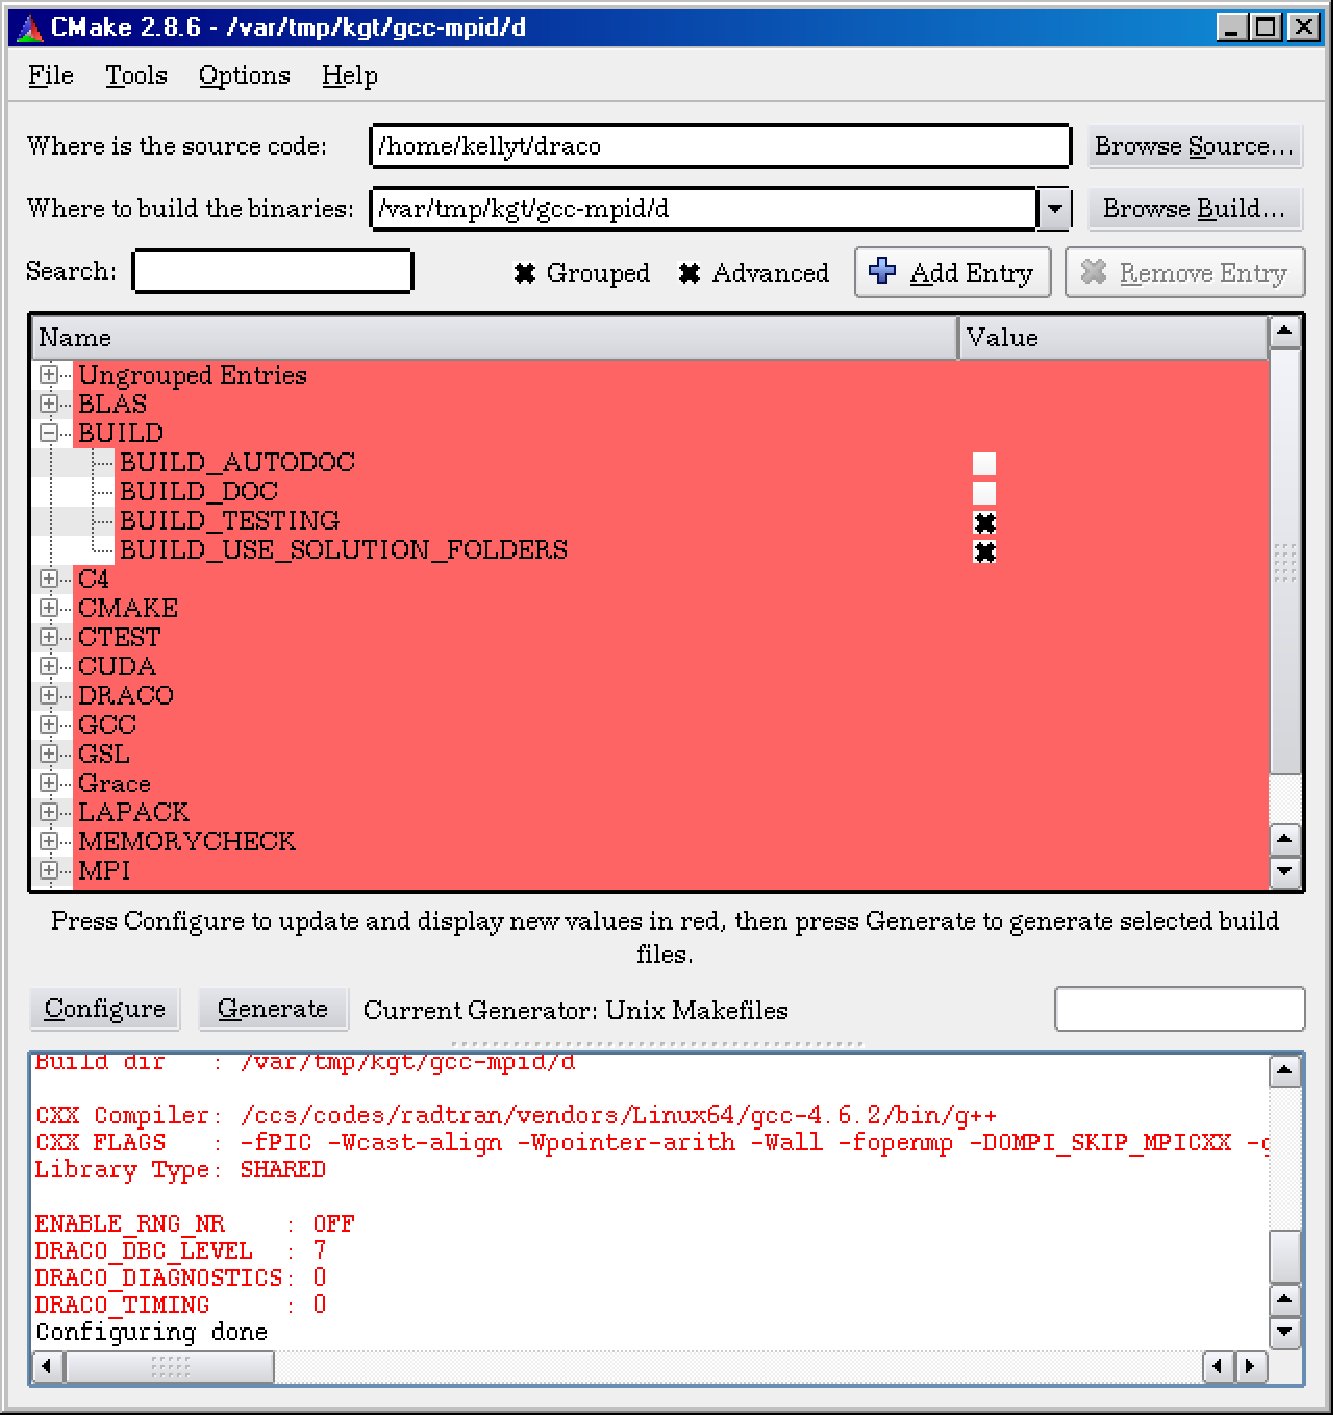
\includegraphics[angle=0,width=5.5in]{fig/cmakegui_defaults}}
  \caption{CMake GUI after populating cache with default values.}
  \label{fig:cmakegui_defaults}
\end{figure}
%

%% ---------------------------------------------------------------------------- %%
\subsection{Configuration Options}
\label{sec:configuration_options}

Because \draco\ has many packages it must support many configurations.
Additionally, some of these options can be matrixed.  For example,
\draco\ can be configured for 64-bit or 32-bit machines, scalar or parallel, with shared libraries or
archived libaries, and so forth.  The options that one gives during the \cmake\ 
configure step specify most of these options. Also, the build
system has built-in intelligence that will try to make the right
choice if incomplete listings for various options are specified.

For the standard set of \cmake\ options, see Ref.~\cite{cmake}.  The full set of configure options may be examined by running the \cmake\ interactive sessions (\comp{ccmake} or \comp{cmake-gui}).  Some options may only appear on specific systems, after specific vendor installations are discovered, or for specific {\it generators}.  This is the reason that you may need to run {\it configure} more than once when using the interactive versions of \cmake.
%For the standard set of configure options, see Ref.~\cite{autoconf}.
%The full set of configure options may be reproduced at the
%command-line by entering
%\begin{verbatim}
%     $ $draco_home/draco_config --help
%\end{verbatim}
%or 
%\begin{verbatim}
%     $ $draco_home/configure --help
%\end{verbatim}
%Note that from this point onward, we will only give examples using
%\dracoconf. 
As mentioned in the previous section, the built-in configure variable, \comp{CMAKE\_INSTALL\_PREFIX}, should be set explicitly (usually to the target directory) by the
user to avoid installation of \draco\ components in \comp{/usr/local/}.  Alternately, the developer may consider the use of \cmake's \comp{DESTDIR} feature (See \href{http://www.cmake.org/Wiki/CMake_FAQ#Does_CMake.27s_.22make_install.22_support_DESTDIR.3F}{CMake FAQ}).

Configuration options come in four forms: \comp{FILEPATH}, \comp{PATH}, \comp{STRING} and \comp{BOOL}\footnote{There are actually variable types in \cmake.  The 5th type is \comp{INTERNAL}, but this type is not available for user manipulation.}.\index{cmake!variable types}   \draco\ policy is to name \comp{BOOL} options prefixed with \comp{ENABLE\_} or \comp{USE\_}, although there are some exceptions to this policy and this policy is not adopted by \cmake\ built-in variables.  Other variable names should be prefixed with a name to provide context.  This provides a sorted in list the \comp{CMakeCache.txt} file and in the \comp{ccmake} interface and it allows groupings to be collapsed in the GUI.  This policy of using prefix context strings is a \cmake\ and a \draco\ policy standard.
Table~\ref{tab:draco-enable} lists the complete set of \comp{BOOL}
\begin{table}
  \caption{List of \comp{BOOL} options that are unique to \draco.}
  \label{tab:draco-enable}
  \begin{center}
    \begin{tabular}{lcp{3in}} \hline\hline
      \multicolumn{1}{c}{Option} & \multicolumn{1}{c}{Default Value} &
      \multicolumn{1}{c}{Description} \\ \hline
                                % --enable-shmem
%      \comp{--enable-shmem} & off & turns on \shmem\ communication
%      library \\
                                % --enable-pcglib
%      \comp{--enable-pcglib} & on & turns off \pcglib \\
                                % --enable-shared
%      \comp{--enable-shared} & off & turns on shared (\comp{.so})
%      libraries \\
%                                % --enable-static-ld
%      \comp{--enable-static-ld} & off & tries to use static
%      (\comp{.a}) libraries for linking \\
%                                % --enable-strict-ansi
%      \comp{--enable-strict-ansi} & on & compiles using \comp{strict}
%      flags for ANSI compliance \\
%                                % --enable-debug
%      \comp{--enable-debug} & off & turns on \comp{-g} option for
%      debugging$^{\text{a}}$ \\ 
%                                % --enable-32-bit
%      \comp{--enable-32-bit} & off & turns on 32-bit compiling on SGIs 
%      \\
\comp{ENABLE\_RNG\_NR} & OFF & Selects the non-reproducible random number generator feature \\
\comp{USE\_OPENMP} & ON & Disables OpenMP pragmas when compiling \draco\ sources \\
\comp{BUILD\_AUTODOC} & OFF & Enables discovery of Doxygen and the \comp{autodoc} build target \\
%\comp{BUILD_DOC} & OFF & Enables building of all \LaTeX\ documentation found in the \comp{doc} directory \\
\comp{BUILD\_TESTING} & ON & Allows developers to omit configuring for and building code found in test directories (disables \ctest\ features) \\
\comp{BUILD\_USE\_SOLUTION\_FOLDERS} & ON & Only available for \sys{Visual Studio} and \sys{X-Code} generators; makes each \draco\ component a solution folder \\
\comp{CMAKE\_VERBOSE\_MAKEFILE}$^{\text{a}}$ & OFF & Forces the make process to echo all commands to the screen during the build process \\
\comp{GCC\_ENABLE\_ALL\_WARNINGS} & OFF & When using gcc, enable more compiler warning features \\
\comp{GCC\_ENABLE\_GLIBCXX\_DEBUG} & OFF &  When using gcc, use alternate glibc library that provides bounds checking and more safety features \\

              \hline\hline
% footnote
      \multicolumn{3}{p{6in}}{$^{\text{a}}${\footnotesize this option is provided by \cmake\ and is not unique to \draco.  It is provided here because it is a commonly used feature.}}
                                % footnote
%      \multicolumn{3}{l}{$^{\text{a}}$the \KCC\ compiler automatically 
%        includes \comp{-g} support for optimization level \comp{K0},
%        see \S~\ref{sec:optimization}.}
    \end{tabular}
  \end{center}
\end{table}
switches that are unique to \draco.  To turn off a switch the user has
two options, \comp{-DENABLE\_SWITCH=OFF} or run an interactive \cmake\ session and toggle the value.  See Ref.~\cite{cmake} for more details concerning \cmake\ variables.

The \comp{PATH}, \comp{FILEPATH} and \comp{STRING} \cmake\ configure options take actual string arguments.
Table~\ref{tab:draco-with} lists commonly used argument based configure options for \draco.  Some of these are restricted to values provided by a drop down list in the GUI.
\begin{table}
  \caption{List of value based options that are unique to \draco.}
  \label{tab:draco-with}
  \begin{center}
    \begin{tabularx}{\linewidth}{
        >{\setlength{\hsize}{1.0\hsize}}X %
        >{\setlength{\hsize}{.6\hsize}}X %
        >{\setlength{\hsize}{.6\hsize}}X  %
%        >{\setlength{\hsize}{1.1\hsize}}X %
        >{\setlength{\hsize}{1.7\hsize}}X}
      \hline\hline
                                % TABLE HEADINGS
      \multicolumn{1}{c}{Option} & \multicolumn{1}{c}{Valid Arguments} 
      & \multicolumn{1}{c}{Default Value} 
%      & \multicolumn{1}{c}{Implied Argument} 
& \multicolumn{1}{c}{Description} \\ 
\hline\hline
%                                % --with-mpi
%      \comp{--with-mpi} & \comp{vendor mpich} & \comp{no} &
%      \comp{vendor} & see \S~\ref{sec:vendor_libs} \\
%                                % --with-mpi-inc
%      \comp{--with-mpi-inc} & \vble{dir} & \cnull &
%      \comp{\$MPI\_\,INC\_\,DIR} & see \S~\ref{sec:vendor_libs} \\ 
%                                % --with-mpi-lib
%      \comp{--with-mpi-lib} & \vble{dir} & \cnull &
%      \comp{\$MPI\_\,LIB\_\,DIR} & see \S~\ref{sec:vendor_libs} \\
%                                % --with-shmem-inc
%      \comp{--with-shmem-inc} & \vble{dir} & \cnull &
%      \comp{\$SHMEM\_\,INC\_\,DIR} & see \S~\ref{sec:vendor_libs} \\ 
%                                % --with-shmem-lib
%      \comp{--with-shmem-lib} & \vble{dir} & \cnull &
%      \comp{\$SHMEM\_\,LIB\_\,DIR} & see \S~\ref{sec:vendor_libs} \\
%                                % --with-sprng
%      \comp{--with-sprng} & \comp{lfg lcg} & \comp{lfg} & \comp{lfg} &
%      see \S~\ref{sec:vendor_libs} \\
%                                % --with-sprng-inc
%      \comp{--with-sprng-inc} & \vble{dir} & \cnull & 
%      \comp{\$SPRNG\_\,INC\_\,DIR} & see \S~\ref{sec:vendor_libs} \\ 
%                                % --with-sprng-lib
%      \comp{--with-sprng-lib} & \vble{dir} & \cnull &
%      \comp{\$SPRNG\_\,LIB\_\,DIR} & see \S~\ref{sec:vendor_libs} \\
%                                % --with-pcglib-lib
%      \comp{--with-pcglib-lib} & \vble{dir} & \cnull &
%      \comp{\$PCGLIB\_\,LIB\_\,DIR} & see \S~\ref{sec:vendor_libs} \\
%                                % --with-c4
%      \comp{--with-c4} & \comp{scalar mpi shmem} & \comp{scalar} &
%      \comp{scalar} & see \S~\ref{sec:c4_lib} \\
%                                % --with-dbc
%      \comp{--with-dbc} & \comp{0,1,...,7} & \vble{default} &
%      \vble{default} & see \S~\ref{sec:dbc} \\
%                                % --with-opt
%      \comp{--with-opt} & \comp{0,1,2,3} & \comp{0} & \comp{0} & see
%      \S~\ref{sec:optimization} \\
%                                % --with-posix
%      \comp{--with-posix} & \vble{posix src. num.} & \comp{199309L} &
%      \comp{199309L} & sets POSIX source version \\
%                                % --with-mips
%      \comp{--with-mips} & \comp{1,2,3,4} & \comp{mips4} & \comp{4} &
%      sets instruction set on SGIs \\
      	
      \comp{NUMDIFF} & \comp{FILEPATH} to \sys{numdiff} & automatic discovery &  tool used by testing system for comparing output to gold standard output. \\
      \comp{VENDOR\_DIR} & \comp{PATH} & empty & location used by build system for auto discovery of vendor software. \\
      \comp{DRACO\_C4} & MPI or SCALAR & MPI$^{\text{a}}$ & see \S~\ref{sec:vendor_libs} \\
      \comp{DRACO\_DBC\_LEVEL} & 0-15 & 7$^{\text{b}}$ &  see \S~\ref{sec:dbc} \\
      \comp{DRACO\_DIAGNOSTICS} & 0-7 & 0 &  see \S~\ref{sec:diagnostics} \\
      \comp{DRACO\_LIBRARY\_TYPE} & STATIC or SHARED & SHARED &  toggle compilation of archive or shared object (DLL) libraries \\
      \comp{DRACO\_TIMING} & 0-2 & 0 &  see \S~\ref{sec:diagnostics} \\
      \comp{DRACO\_VERSION} & \comp{STRING} & hard coded$^{\text{c}}$ & string that represents the current version of \draco.  This is embedded into the installed \draco\ products. \\
      \comp{DRACO\_VERSION\_FULL} & \comp{STRING} & hard coded$^{\text{c}}$ & string that represents the current version of \draco.  This is embedded into the installed \draco\ products. \\
      
      \hline
      
      \comp{CMAKE\_BUILD\_TYPE} & Debug or Release or RelWithDebInfo or MinSizeRel & Debug & choose type build type; default compiler flags are triggered based on this selection. \\
      \comp{CMAKE\_CXX\_COMPILER} & \comp{FILEPATH} to compiler & \comp{\$ENV{CXX}} & \cpp\ compiler chosen for build.\\
      \comp{CMAKE\_C\_COMPILER} & \comp{FILEPATH} to compiler & \comp{\$ENV{CC}} & C compiler chosen for build. \\
      \comp{CMAKE\_Fortran\_COMPILER} & \comp{FILEPATH} to compiler & \comp{\$ENV{FC}} & Fortran compiler chosen for build. \\
      \comp{CMAKE\_INSTALL\_PREFIX} & \comp{PATH} & \comp{\${BINARY\_DIR} /target} & location for installing \draco (libraries, headers, executables, etc). \\
      
      \hline
      
      {\it VENDOR\_VARIABLE} & varies & automatic discovery & configuration of vendors is done automatically by the \draco\ build system. See \S~\ref{sec:vendor_libs}. \\
      
      \hline\hline
% footnote
      \multicolumn{4}{p{6in}}{$^{\text{a}}${\footnotesize MPI if \sys{MPI} can be found, otherwise SCALAR.}} \\
      \multicolumn{4}{p{6in}}{$^{\text{b}}${\footnotesize The default is 7 for DEBUG builds and 0 for RELEASE (optimized) builds.}} \\
      \multicolumn{4}{p{6in}}{$^{\text{c}}${\footnotesize The version string is built from hard coded values \comp{DRACO\_VERSION\_MAJOR} and \comp{DRACO\_VERSION\_MINOR} hard coded in the top level \comp{CMakeLists.txt}. The patch revision number is set to the configure date for development builds.  Scripts used for releases set the patch version manually.}} 
    \end{tabularx}
  \end{center}
\end{table}
Notice that the build system will automatically populate all fields with default values so that \draco\ can be configured without supplying values for every possible feature.
%\comp{--with} can be used without arguments.  In this case
%an implied argument is assumed by configure.  Thus, \comp{--with}
%options have a default value and an implied argument value.  In the
%first case, a default value is inferred by configure if the
%\comp{--with} option is absent.  In the latter case, an implied
%argument is provided if the \comp{--with} option is present but does
%not specify an argument.
For example, the following two configurations are equivalent because the default value for \comp{DRACO\_C4} is \comp{MPI} if \sys{MPI} can be found on the local system.
\begin{verbatim}
     $ cmake -DDRACO_C4=MPI $draco_home
     $ cmake $draco_home 
\end{verbatim}
In each case, the \cfour\ package is configured for parallel operation with \sys{MPI}.  In the first
case an explicit argument is given.  In the second case  the default value for
\comp{DRACO\_C4} is used.  Not all cases have the same defaults for
options and arguments.  An example is the \comp{MPI\_LIBRARY}
option.  The default is the value returned from the \cmake\ built-in function \comp{find\_package(MPI)}.  For more information about configuring and auto-discovery of vendor software see \S~\ref{sec:vendor_libs} below.
% If the option is given without an argument, configure sets
%\comp{--with-mpi-inc=\$MPI\_\,INC\_\,DIR}. In general, the class of
%\comp{--with} options that load external libraries work in this
%fashion.  Most other \comp{--with} options have the same defaults as
%implied arguments.  On a final note, we do not recommend the practice
%of setting \comp{--without} because \comp{--with} options are not
%meant for binary-type operations.  An exception to this rule is the
%vendor-associated options described in \S~\ref{sec:vendor_libs}.


%% ---------------------------------------------------------------------------- %%
\subsubsection{Vendor Libraries}
\label{sec:vendor_libs}

\draco\ uses external vendors whenever possible to reduce the ammount
of code development required by \draco\ package developers.  The
following vendors are used by \draco:
\begin{itemize}
\item \mpi\ communication library, see \S~\ref{appsec:mpi};
\item \pkg{GSL}, GNU Scientific Library, provides a wide range of mathematical routines such as random number generators, special functions and least-squares fitting, see \S~\ref{appsec:gsl};
\item \pkg{LAPACK} and \pkg{BLAS} provide optimized linear algebra algorithms, see \S~\ref{appsec:lapack};
\item \pkg{CUDA} provides support for running threads on Graphic Processing Units, GPUs, see \S~\ref{appsec:cuda};
\item \pkg{DaCS} provides support for running threads on IBM cell processing units, see \S~\ref{appsec:dacs};
\item \pkg{XMGRACE} provides a 2D plotting capability, see \S~\ref{appsec:grace};
%\item \shmem\ communication library, see \S~\ref{appsec:shmem};
%\item \sprng\ random number library, see \S~\ref{appsec:sprng};
%\item \pcglib\ parallel conjugate gradient solver, see  \S~\ref{appsec:pcglib}.
\end{itemize}\index{vendor!MPI}\index{vendor!GSL}\index{vendor!LAPACK}\index{vendor!CUDA}\index{vendor!Grace}
Vendors are accessed through the \draco\ build system via automatic discovery.  
%using defined \comp{--with} and \comp{--enable} tags in \autoconf.
Table~\ref{tab:vendortags} lists the environment and build system variables that can be manipulated by the developer to alter the discovery process.
\begin{table}
  \caption{Environment and build system variables used to specify vendors in \draco.  See Tables~\ref{tab:draco-enable} and \ref{tab:draco-with} for variable defaults.}
  \label{tab:vendortags}
  \begin{center}
    \begin{tabular}{lap{3.5in}}
    \hline\hline
      \multicolumn{1}{c}{Vendor} & \multicolumn{1}{c}{Variable} & \multicolumn{1}{c}{Details} \\
      \hline
% MPI
      \mpi$^{\text{a}}$ & ENV\{PATH\} & The build system looks for \comp{mpirun} in the current \comp{PATH}. \\
      & MPIEXEC & The full path to the \comp{mpirun} program.  This may need to be set manually if the program has a non standard name like \comp{aprun}. \\
      & MPIEXEC\_NUMPROC\_FLAG & The string used to specify then number of processors to use. Defaults to \comp{'-np'}. \\ 
      & MPI\_C\_LIBRARIES & Manually specify the full paths to \sys{MPI} libraries. \\
      & MPI\_CXX\_LIBRARIES  & \\
      & MPI\_Fortran\_LIBRARIES & \\
      & MPI\_C\_INCLUDE\_PATH & Manually specify the full path to the \sys{MPI} include directory. \\
      & MPI\_CXX\_INCLUDE\_PATH & \\
      & MPI\_Fortran\_INCLUDE\_PATH & \\
      \hline
% LAPACK/BLAS      
      \pkg{LAPACK} & BLA\_STATIC & Look for archive (static) \pkg{LAPACK} and \pkg{BLAS} libraries. Default is ON. \\
      & BLA\_VENDOR & Use a particular type of \pkg{LAPACK} installation like \sys{ATLAS} or \sys{Intel10\_64lp\_gf\_sequential}$^{\text{b}}$. \\
      & ENV\{LD\_LIBRARY\_PATH\} & To help the build system find \pkg{LAPACK}, ensure that the library location is appended to this environment variable. \\ 
      & ENV\{LAPACK\_LIB\_DIR\} & To load a specific \pkg{LAPACK}, ensure this variable is set to the desired location. \\
      \hline
% GSL
      \pkg{GSL} & ENV\{GSL\_INC\_DIR\} & Help the build system find the desired installation by setting this environment variable. \\
      &  ENV\{GSL\_LIB\_DIR\} & Help the build system find the desired installation by setting this environment variable. \\
      \hline
% XMGRACe
      \pkg{XMGrace} & ENV\{GRACE\_INC\_DIR\} & Help the build system find the desired installation by setting this environment variable. \\
      &  ENV\{GRACE\_LIB\_DIR\} & Help the build system find the desired installation by setting this environment variable. \\
      \hline
% CUDA
     \pkg{CUDA}$^{\text{c}}$ &  ENV\{PATH\} & The build system looks for \comp{nvcc} in the current \comp{PATH}. \\
     & CUDA\_NVCC\_FLAGS & Modify the \comp{nvcc} compiler flags. Default is \comp{'-arch=sm\_21'}. \\
     & CUDA\_TOOLKIT\_ROOT\_DIR & If the build system cannot find \comp{nvcc}, the developer must set this location to enable \pkg{CUDA}. \\
     & CUDA\_BIN\_PATH & To use a non-standard location, set this before running \cmake. \\
     
% SHMEM
%      \shmem & --enable-shmem \\
%      & --with-shmem-inc \\
%      & --with-shmem-lib \\ \hline
% SPRNG
%      \sprng & --with-sprng \\
%      & --with-sprng-inc \\
%      & --with-sprng-lib \\ \hline
% PCGLIB
%      \pcglib & --enable-pcglib \\
%      & --with-pcglib-lib \\
      \hline\hline
      % footnotes
      \multicolumn{3}{p{6in}}{$^{\text{a}}${\footnotesize Run \comp{'cmake --help-module FindMPI'} for more details on the discovery process for \pkg{MPI}.}} \\
      \multicolumn{3}{p{6in}}{$^{\text{b}}${\footnotesize To obtain a list of support installations of \pkg{LAPACK}, see the documentation for \cmake's \comp{FindLAPACK.cmake} module (try \comp{'cmake --help-module FindLAPACK'}).}} \\
      \multicolumn{3}{p{6in}}{$^{\text{c}}${\footnotesize Run \comp{'cmake --help-module FindCUDA'} for more details on the discovery process for \pkg{CUDA}.}} \\
    \end{tabular}
  \end{center}
\end{table}
Tables~\ref{tab:draco-enable} and \ref{tab:draco-with} list additional controls that can manipulate how each vendor is used in \draco.  Details on how to use
these variables are given below.

\draco\ vendor libraries are of two types; \latin{required} and
\latin{optional}.  The type classification for each vendor is found in
Table~\ref{tab:vendor}.  \draco\ treats vendors according to the
following rules:
\begin{enumerate}
\item Required vendor libraries are on by default and the configuration will {\bf fail} if the libraries cannot be located;
\item Optional vendor libraries are on by default but the configuration will {\bf pass} if the libraries cannot be located.
\end{enumerate}
For example, \pkg{GSL} is a required vendor.  If \pkg{GSL} cannot be found, the project will not be configured and  cannot be built.  If the optional vendor \pkg{XMGrace} cannot be found, the configuration will be successful, but the \draco\ component \pkg{plot2D} will be omitted because it requires \pkg{XMGrace}.  Finally, if the optional vendor \pkg{MPI} cannot be found the configuration will be sucessful, but the \cfour\ component will be built with the \comp{SCALAR} option instead of \comp{MPI}.  Review Table~\ref{tab:depends} to determine what components may be omitted when vendor libraries are not found. This concept applies to all vendor libraries.

%We note that these rules are applied on a package-by-package basis.
%For example, \sprng\ is only required for \rng; thus, \sprng\ is on in
%the \rng\ and \imc\ packages (see Table~\ref{tab:depends}).  It is
%undefined everywhere else.  

%As illustrated in Table~\ref{tab:vendortags}, vendor options are set
%by the following three configure tags:
%\begin{enumerate}
%\item \comp{--with-\vble{vendor}} (\comp{--enable-\vble{vendor}})
%  turns the vendor on or off.  If the vendor has options (e.g.
%  \comp{--with-mpi}) then \comp{--with} is used.  If the vendor is
%  simply on or off (e.g.  \comp{--enable-shmem}) then \comp{--enable}
%  is used.
%\item \comp{--with-\vble{vendor}-inc} overrides the default \soft{cpp}
%  search locations for header files if the vendor is on.
%\item \comp{--with-\vble{vendor}-lib} overrides the default search
%  path (\ldlib) for libraries if the vendor is on.
%\end{enumerate}
%Optional vendors may be turned on simply by setting
%\comp{--with-\vble{vendor}-inc} or \comp{--with-\vble{vendor}-lib}.
%If these tags are set without setting \comp{--with-\vble{vendor}} then
%the optional library is turned on, and \comp{--with-\vble{vendor}}
%takes the value of its implied argument.  Libraries that use a
%\comp{--enable} tag are simply on in this case.  Naturally, the
%headers and libraries are searched in the directories given by
%\comp{--with-\vble{vendor}-inc} and \comp{--with-\vble{vendor}-lib}.
%For required vendors, setting \comp{--with-\vble{vendor}-inc} or
%\comp{--with-\vble{vendor}-lib} simply changes the default search
%locations for headers and libraries as explained above.

% We note that if an optional vendor is not found by the build system then
% the packages that depend on these vendors will not build.  
%%In other
%%words, required vendors need not be turned off even if the packages
%%that use them are not part of a specific \draco\ distribution.
% \draco\ knows what packages require what vendors, so optional vendor libraries that are missing
% in a particular distribution will have no effect on the rest of the packages.

%% ---------------------------------------------------------------------------- %%
\subsubsection{C4 Package Options}
\label{sec:c4_lib}

\cfour\ is \draco's parallel communication package.  It uses \mpi\ 
%either \mpi\ or \shmem\ 
to perform message passing operations.  Therefore, \cfour\ is intimately connected to the \mpi\ 
%and \shmem\ 
vendor.  The \cmake\ variable \comp{DRACO\_C4} determines how \cfour\ should be configured. 
The default option and implied argument is \comp{DRACO\_C4=MPI} when an \sys{MPI} installation is located by the build system.  However, if \cfour\ is set to \comp{SCALAR} 
then that vendor will be turned off with their implied
argument settings.  Of course, the implied arguments can be overridden by using the \mpi\ 
% or \shmem\ 
build system variables from
Table~\ref{tab:vendortags}.  In summary, if \cfour\ is set to
\comp{mpi}, those libraries will be turned on with all 
default settings.  However, any of the defaults can be changed by
using the \mpi\ vendor tags that are listed in
Table~\ref{tab:vendortags}. 

Some \sys{MPI} installations for ASC hardware are not fully supported by \cmake's built in \comp{FindMPI.cmake} routines.  
This is the case for \latin{Cielito} and \latin{Cielo}.  For these systems the \draco\ build system
employs a \latin{toolchain} file to aid in the selection of appropriate compilers and \sys{MPI} environment variables.  
To configure \draco\ on these systems use a command similar to
\begin{verbatim}
     $ cmake -DCMAKE_TOOLCHAIN_FILE=$draco_home/config/Toolchain-catamount.cmake \
             $draco_home
\end{verbatim}
The \comp{CMAKE\_TOOLCHAIN\_FILE} command line argument should appear first in the list of arguments provided to \cmake.
It is recommended that developers review the \comp{Toolchain-catamount.cmake} file to observe how the compilers and \sys{MPI}
libraries are set before compiling on either of these systems.

%% ---------------------------------------------------------------------------- %%
\subsubsection{Design-by-Contract}
\label{sec:dbc}\index{Design-by-Contract}

The \comp{DRACO\_DBC\_LEVEL} variable controls \draco's Design-by-Contract
(DBC) machinery\index{Design-by-Contract}\index{DBC}.  DBC support ranges from \comp{0} (lowest) to
\comp{15} (highest).  The value is a bit mask similar to that used by the \sys{UNIX} command \comp{chmod}, \comp{+1} turns on \comp{Require}, 
\comp{+2} turns on \comp{Check}, \comp{+4} turns on \comp{Ensure} and \comp{+8} disables exception throwing.  If all options are activated, the  Design-by-Contract is 15. Normal Debug builds use \comp{DRACO\_DBC\_LEVEL=7} where all Design-by-Contract checks are active and exceptions are thrown when a contract is violated.
Table~\ref{tab:dbc} shows the DBC level for various settings of \comp{DRACO\_DBC\_LEVEL}. \index{configure options!DRACO\_DBC\_LEVEL}
\begin{table}
  \caption{DBC support in \draco.}
  \label{tab:dbc}
  \begin{center}
    \begin{tabular}{ca} \hline\hline
      \multicolumn{1}{c}{DBC Setting} & \multicolumn{1}{c}{DBC Functions} \\ \hline
      0 & None\\
      1 & Require, Remember \\
      2 & Check, Remember \\
      3 & Check, Require, Remember \\
      4 & Ensure, Remember \\
      5 & Ensure, Require, Remember \\
      6 & Ensure, Check, Remember \\
      7 & Ensure, Check, Require, Remember \\ 
      8 & None \\
      9 & Require, Remember, NoThrow \\
      10 & Check, Remember, NoThrow \\
      11 & Check, Require, Remember, NoThrow \\
      12 & Ensure, Remember, NoThrow \\
      13 & Ensure, Require, Remember, NoThrow \\
      14 & Ensure, Check, Remember, NoThrow \\
      15 & Ensure, Check, Require, Remember, NoThrow \\ 
      \hline\hline
    \end{tabular}
  \end{center}
\end{table}
If this option is not explicitly set by the developer (\comp{DRACO\_DBC\_LEVEL} is not defined) then the
\dsxx\ package automatically sets DBC to \comp{7}, its most aggressive
setting, for \sys{Debug} configrations.  For \sys{Release} configurations, the DBC will be defaulted to \comp{0}, no DBC checking.  
For more information on the \dsxx\ package DBC and assertion components, see the \dsxx\ source documentation.

%% ---------------------------------------------------------------------------- %%
\subsubsection{Diagnostics}
\label{sec:diagnostics}\index{configure options!DRACO\_DIAGNOSTICS}\index{configure options!DRACO\_TIMING}

The \comp{DRACO\_DIAGNOSTICS} and \comp{DRACO\_TIMING} build variables control \draco's \pkg{diagnostic} machinery.  The purpose of this component is allow other \draco\ components to collect and report diagnostic data during runtime.  When \comp{DRACO\_DIAGNOSTICS} feature is turned off, the inserted diagnostic code does not cause any performance penalty because it is a compile time feature.  The same is true for \comp{DRACO\_TIMING} which focuses on profiling and reporting perfomance timing statistics.  The allowed values for each of these build variables are bit masks as explained in \S~\ref{sec:dbc}.  Tables~\ref{tab:ddiagnostics} and \ref{tab:dtiming} provide a description for variouls settings.
\begin{table}
  \caption{Diagnostics support in \draco.}
  \label{tab:ddiagnostics}
  \begin{center}
    \begin{tabular}{ca} \hline\hline
      \multicolumn{1}{c}{Diagnostic Setting} & \multicolumn{1}{c}{Diagnostic level description} \\ \hline
      0 & all off\\
      1 & low cost diagnostics enabled \\
      2 & moderate cost diagnostics enabled \\
      3 & moderate and low cost diagnostics enabled\\
      4 & high cost diagnostics enabled\\
      5 & high and low cost diagnostics enabled \\
      6 & high and moderate cost diagnostics enabled \\
      7 & all diagnostics enabled \\ 
      \hline\hline
    \end{tabular}
  \end{center}
\end{table}
%
\begin{table}
  \caption{Timing diagnostic support in \draco.}
  \label{tab:dtiming}
  \begin{center}
    \begin{tabular}{ca} \hline\hline
      \multicolumn{1}{c}{Timing Diagnostic Setting} & \multicolumn{1}{c}{Timing diagnostic functions} \\ \hline
      0 & all off\\
      1 & TIMER, TIMER\_START, TIMER\_STOP and TIMER\_RECORD available \\
      2 & all functions available, including TIMER\_REPORT \\
      \hline\hline
    \end{tabular}
  \end{center}
\end{table}

%% ---------------------------------------------------------------------------- %%
\subsubsection{Optimization}
\label{sec:optimization}\index{optimization}

The optimization flags\index{optimization} for the \comp{CXX}, \comp{CC} and \comp{FC} \index{configure option!CXX} \index{configure option!CC}\index{configure option!FC} compilers have default values established 
based on the compiler vendor and the selected build type (\comp{Release}, \comp{Debug}, etc.).  These flags
are established in \draco\ build system's configuration files \comp{config/}\vble{arch\_compiler\_vendor}\comp{.cmake} 
(e.g.: \comp{config/unix-g++.cmake} or \comp{config/windows-cl.cmake}).  In general, \comp{Release} configurations will use optimization flags like \comp{-O3 -funroll-loops} and \comp{Debug} configurations will include debug symbols and no optimization, \comp{-g -O0}.  The \comp{RelWithDebInfo} configuration uses a mixture of flags trying to produce an optimized configuration that still has the debug symbols.  \draco\ policy to keep the source code as close to the language standard as possible.   To aid the developer, the \comp{Debug} configurations impose compiler flags that will increase the warning level and verbosity during the compilation.  For example, when using the \sys{g++} compiler the flags \comp{'-ansi -pedantic -Wcast-align -Wpointer-arith -Wall'} are used for \comp{Debug} configurations. In general, \comp{Release} builds use the most aggressive optimizations that provide reliable and consistent results.

%The optimization flags for \KCC, the \cpp\ compiler of choice for
%\draco, has some unique options.  Specifically, the lowest level of
%optimization, \comp{--with-opt=0}, which is given by default and by
%implied argument, automatically sets the \KCC\ compile-line flag,
%\comp{+K0}.  The \comp{+K0} option implicitly includes the debug flag
%\comp{-g}.  Thus, when \comp{--with-opt=0} the debug flag
%(\comp{--enable-debug}) does not have to included.  \draco\ has
%built-in intelligence that will turn off the \comp{-g} flag if the
%\KCC\ optimization is set to \comp{0}.  The \comp{-g} flag will be
%included for any optimization setting greater than \comp{0}.

%%---------------------------------------------------------------------------%%

\section{Building Draco}
\label{sec:building_draco}

After configuration, building \draco\ is mostly straightforward.  For \sys{UNIX} \sys{Makefile} build configurations, 
one simply enters the binary directory, or a component's binary
subdirectory, and runs \gmake.  The \draco\ Makefiles include all of
the standard targets provided by \cmake.  For more detail, see ref.~\cite{cmake}. The most commonly used targets are \comp{all} and \comp{install}.  \index{build target!all}\index{build target!install}
The \draco\ build system takes full advantage of multi-core architectures allowing multithreaded compilation of \draco.  
To take advantage of this features use the \comp{'-j N'} option of \gmake.  The recommended value for the number of concurrent threads, 
\comp{N}, is 50\% oversubscription of the number of available cores (i.e.: 24 for a 16-core machine). Examples of various builds are reserved
until \S~\ref{sec:examples}.\index{compile!parallel}

For other build environments like \sys{Eclipse} or \sys{XCode}, \cmake\ provides a solution configuration that can be loaded into the IDE.  Use the 
build environment's normal methods for compiling the \comp{ALL\_BUILD} target.

%% ---------------------------------------------------------------------------- %%
\subsection{Building and Installing}

Building and installing \draco\ is specific to each generated project type.  The following subsections provide details for the most commonly used development environments.

\subsubsection{Unix Makefiles}

To build and install \draco\ simply enter the \comp{\vble{target}/draco/} binary directory and run \comp{'gmake -j'}.  At this
level, \gmake\ will enter each subdirectory under \comp{\vble{target}/draco/} and do a full build.
% followed by an install.  
The default targets in subdirectories under \comp{\vble{target}/draco/} are the same as at the top level.  It should be noted that the default target, \comp{all}, does not run unit tests or install \draco\ libraries or headers.  You must run \comp{'make -j install'} to tell the build system to copy the installable artifacts to the prefix directory.
%  Table~\ref{tab:gmake} shows   the default targets at various
%\begin{table}
%  \caption{Default targets for \gmake\ at each directory level.  The
%    \comp{draco/} directory is a subdirectory of the target directory.}
%  \label{tab:gmake}
%  \begin{center}
%    \begin{tabularx}{\linewidth}{
%        >{\setlength{\hsize}{.85\hsize}}L %
%        >{\setlength{\hsize}{.75\hsize}}L %
%        >{\setlength{\hsize}{1.4\hsize}}X}
%      \hline\hline
%      \multicolumn{1}{Y}{\draco\ directory} &
%      \multicolumn{1}{Y}{Default Target} &
%      \multicolumn{1}{Y}{Description} \\ \hline
%                                % draco/
%      draco/ & install: & builds and installs all sub-directories \\
%                                % draco/src
%      draco/src & install: & builds and installs all \comp{src/}
%      sub-directories \\
%                                % draco/src/pkg
%      draco/src/\vble{pkg} & lib\vble{pkg}.\vble{suffix}: & builds the
%      library for \vble{pkg} \\
%                                % draco/src/pkg/test
%      draco/src/\vble{pkg}/test & \${test\_\,alltarget}: & builds all of
%      the test executables \\
%                                % draco/doc
%      draco/doc & install dvi: & builds and installs main \draco\
%      manual \\
%                                % draco/doc/sub-doc
%      draco/doc/\vble{sub-doc} & \${manual} & builds the manual
%      (\comp{.dvi}) in the \vble{sub-doc/} directory \\
%                                % draco/tools
%      draco/tools & install: & installs tools into the \comp{libexec}
%      directory specified by \comp{--prefix} \\
%      \hline\hline
%    \end{tabularx}
%  \end{center}
%\end{table}
%levels of the target directory tree.  
% If \gmake\ is run at levels lower than the \comp{\vble{target}/draco/src/} directory, the user must be aware of package dependencies.  
% For example, \cfour\ cannot be built if \dsxx\ has not been built and installed.  Thus, the general user should avoid manual builds of packages at the
% \comp{\vble{target}/draco/src/\vble{pkg}/} level.  At higher levels, \draco\ knows how to build packages in the proper order.

\subsubsection{Eclipse}
To be completed later.

\subsubsection{XCode}
To be completed later.

\subsubsection{Visual Studio}
To be completed later.

\subsubsection{Running the Tests}

Each \draco\ component provides a full suite of unit tests that demonstrate and check the component algorithm's capabilities.  \index{tests!executing}
To run the tests, run \ctest\ from any location in the binary directory.  
If \ctest\ is run from the top level, all unit tests will be run.  
If run from a component subdirectory, only the tests for that component will be executed.  
The \draco\ build system knows how to run the unit tests in parallel taking advantage of all available hardware resources.  
It is recommended that the \ctest\ command be issued with the \comp{'-j N'} option, where \comp{N} is the number of concurrent threads that should be used.  
For testing purposes, it is better to avoid over-subscription of the machine's hardware.

\ctest\ provides many options for running tests: selecting a subset of tests to run; running with different output verbosity, etc.  The developer should review the \ctest\ documentation found at Ref.~\cite{cmake} and by using the \comp{'ctest --help'} command.  In particular, the \comp{-VV} options selects full verbosity for tests and the \comp{-R} option selects all tests whose names match a provided regular expression.  It is \draco\ policy that tests names will provide both the component name and the number of MPI ranks used (if any) in the test name.  This policy allows the developer to run all \cfour\ tests by using the command\index{tests!options}
\begin{verbatim}
     $ ctest -R c4
\end{verbatim}
or all 4 processor MPI tests could be selected by the command:
\begin{verbatim}
     $ ctest -R _4
\end{verbatim}
A list of available test can be obtained using the \comp{-N} option to \ctest.

\subsubsection{Additional Observations and Features}

At each target directory level the \draco\ build system knows all of the component
dependencies so the developer can start the build at any place in the binary tree. 
For example, when compiling from the \cfour\ component directory, the build system will check to see if the \dsxx\ library has been compiled.  
If not, then the \dsxx\ library will be built before compilation of \cfour\ sources begins.  
Even in this situation the build system remains fully aware of threading and it is recommended that a parallel build process be performed unless the developer 
is trying to debug a build system error.   
This aspect of the build system is a feature for \draco\ developers.  
It allows the developer to only compile or recompile sources that are required for building the desired target.  
One drawback is that other components in parallel directories may be modified during a targeted compile and the developer should remain aware of 
these dependencies as  illustrated in Fig.~\ref{fig:level} and are listed in Table~\ref{tab:depends}.
%
%Thus, \cfour\ simply checks to see if \dsxx\ has been
%installed.  If \dsxx\ does not exist in the install location specified
%by \comp{--prefix} then \gmake\ will end.   It gives developers the
%flexibility to modify code in a package and test it without affecting
%other packages that may depend on that code.  One drawback is that
%users must be aware of the package dependencies when performing manual
%builds.  These dependencies are

%This is done to conform to the GNU Standard, which states that tests should not be dependent upon installation.  The \comp{check} target uses \dejagnu\ to generate test 
%output data and results.  For more information, see
%ref.~\cite{dejagnu}.  A future \draco\ document will describe the
%details of \draco\ regression testing.

An additional feature of the \draco\ build system is that \draco\ will automatically rerun the \cmake\ configuration step if any of the configuration system files have been modified.  
Thus, if \comp{CMakeLists.txt} or any of the files from the \comp{config} source directory are changed then the build process will first reconfigure the entire project.  

%% ---------------------------------------------------------------------------- %%
\subsection{Build Targets}
\index{build target!all}
\index{build target!install}
\index{build target!check}
\index{build target!clean}
\index{build target!rebuild\_cache}
\index{build target!test}
\index{build target!edit\_cache}
\index{build target!Experimental}
\index{build target!help}

A detailed discussion of all the build targets provided by \cmake~\cite{cmake} is beyond the scope of this text. 
What follows is a brief description of the build targets in \draco\ and what operations they perform.\index{build:targets}
\begin{description}
\item[\comp{all}]\index{gmake!target!all} (default) build all products at the current level and in all subdirectories.  If configuration files have been modified, rerun \cmake\ to reconfigure the project before compilation begins.
\item[\comp{install}]\index{gmake!target!install|textbf} build all products at the current level and in all subdirectories; then install the products in the locations specified by \comp{CMAKE\_INSTALL\_PREFIX}.  All build products are compiled before any are installed. 
\item[\comp{check}]\index{gmake!target!check|textbf} build all products at the current level and in all subdirectories; then run \ctest\ to execute all unit tests.  This target does not install any products (this behavior is different than older versions of \draco).
%\item[\comp{install dvi}]\index{gmake!target!install dvi|textbf}
%  \gmake\ will build and install the main \draco\ manual when this is
%  run from the \comp{draco/} or \comp{draco/doc/} directories.  When
%  this target is run from a \comp{draco/doc/\vble{sub-doc}/} directory
%  it will build the \vble{sub-doc} manual and install it.
%\item[\comp{dvi}]\index{gmake!target!dvi|textbf} \gmake\ will build
%  the manual in the directory where this target is run.  In
%  \comp{draco/doc/} it will build the main manual.  In
%  \comp{draco/doc/\vble{sub-doc}/} it will build the \vble{sub-doc}
%  manual.
\item[\comp{clean}]\index{gmake!target!clean|textbf} clean the compiled files (\comp{*.o}, libraries and executables) from the target sub-directories.
\item[\comp{rebuild\_cache}]\index{gmake!target!rebuild\_cache} rerun the \cmake\ configure process and regenerate all project files (e.g.: \comp{Makefiles}, \comp{config.h}, etc.).
\item[\comp{edit\_cache}]\index{gmake!target!edit\_cache} run the \cmake\ editor to allow the developer to edit the configuration variables. 
\item[\comp{test}]\index{gmake!target!test} run \ctest\ to execute all unit tests.
\item[\comp{Experimental}]\index{gmake!targets!Experimental} configure, compile, run the tests and submit the results to the \draco\ \cdash\ dashboard.
\item[\comp{Lib\_}\vble{pkg}]\index{gmake!targets!Lib\_pkg} Compile the library for \draco\ component \vble{pkg}.
\item[\comp{Ut\_}\vble{pkg\_test}\comp{\_exe}]\index{gmake!targets!Ut\_pkg\_test\_exe} Compile the unit test executable for test \vble{test} for the \draco\ component \vble{pkg}.
\item[\comp{help}] provides a list of available targets.
\end{description}
These targets have been designed to satisfy the needs of users, who
perform one-time global builds, and developers, who perform multiple
local builds.

%%---------------------------------------------------------------------------%%

\section{Recommended Practices}

Although \draco\ can be configured and built in any number of ways, we 
have a set of ``standard'' recommended practices that are followed by
\draco\ team members.  This methodology for configuring and
building \draco\ is summarized in the following steps:
\begin{enumerate}
\item Checkout a version of \draco\ from \svn; the location of which is \dracohome.
\item Make a target directory that appropriately describes the configuration options; 
we call this directory \comp{\vble{target}/}.
\item Make a \comp{draco/} binary subdirectory under the target directory,
  ie. \comp{\vble{target}/draco/}.
\item Run \cmake\ in \comp{\vble{target}/draco/} with the appropriate options for this
  configuration.  Set \comp{-DCMAKE\_}\-\comp{INSTALL\_}\-\comp{PREFIX=\vble{target}/}. Thus, the
  configure line is:
  \begin{alltt}
    $ cmake -DCMAKE_INSTALL_PREFIX=`pwd`/.. \vble{options} $draco_home 
  \end{alltt}
\item Run \gmake\ in \comp{\vble{target}/draco/};
\begin{verbatim}
    $ gmake -j install
\end{verbatim} % $
  This step will build and install all of the \draco\ products from
  each subdirectory under \comp{\vble{target}/draco/}.  The headers
  will be installed in \comp{\vble{target}/include/}.  The libraries
  will be installed in \comp{\vble{target}/lib/}. 
  And the executables will be installed in \comp{\vble{target}/bin/}.
  %And, the package-dependent executables will be installed in \comp{\vble{target}/libexec}.
\end{enumerate}
This procedure simplifies adding an external code system that uses,
and is based on, \draco.  For example, \clubimc\ uses \draco\ as a
build-model template.  Thus, we can add a \comp{\vble{target}/clubimc}
directory and configure, build, and install \clubimc\ in the same
location as \draco\ products.  Details on this process are given in
\S~\ref{sec:emulating}. 

%%---------------------------------------------------------------------------%%

\section{Examples}
\label{sec:examples}

To illucidate some of the concepts that we have described in this
chapter, we proceed to show some configuration and build examples.
The following examples give a cross section of the processes that
\draco\ users and developers will use.\index{build!examples}
\begin{cexa}
  \label{ex:basic}
  Build a scalar version of \draco\ on a \sys{Linux} platform using the \sys{Makefile} generator.  
  %\sprng\ headers are in the \soft{cpp} include path, and \sprng\ and \pcglib\ libraries are found in \ldlib.  
  \pkg{GSL} libraries are found in \ldlib.
  The \draco\ source directory is \comp{/usr/tmp/joe/draco}.  
  We want \draco\ installed in \comp{/usr/local/draco}.
\end{cexa}
\begin{proof}[Solution to \ref{ex:basic}]
  First, we need to make a target directory.  In
  \S~\ref{sec:running_configure_prepare} we advised not to use the source
  directory as the build directory.  We will follow this policy and
  make our target directory \comp{draco\_\,target}:
\begin{verbatim}
     $ cd /usr/local/draco
     $ mkdir draco_target
\end{verbatim}
  Note that we could have created a directory named \comp{draco/} instead of \comp{draco\_\,target/}.
  We used a different name to illustrate the independence of the target-build directory.  Now, we configure
  \draco\ according to the specification in Ex.~\ref{ex:basic}.  This
  configuration is scalar so we must specify alternate settings for
  \cfour.  Additionally, all of the required vendors are located in
  default locations.
\begin{verbatim}
     $ cd draco_target
     $ cmake -DCMAKE_INSTALL_PREFIX=`pwd`/.. -DDRACO_C4=SCALAR \
             /usr/tmp/joe/draco/draco_config
\end{verbatim}
  All other defaults are used except the explicit setting for \comp{DRACO\_C4}.
  Finally, we want to do a build and install of all \draco\ products;
  thus, according to \S~\ref{sec:building_draco}, we must enter
\begin{verbatim}
     $ gmake -j install
\end{verbatim} % $
  Generally, it is better run the build (\comp{all} target and then run the unit tests via \ctest\
  before running the \comp{install} target.  This gives the develper a chance to ensure that all tests
  pass before the build is installed.
\begin{verbatim}
     $ make -j 
     $ ctest -j
     $ make -j install
\end{verbatim} %   
\end{proof}

Example~\ref{ex:basic} is straightforward.  We will now give a series
of examples and solutions that involve more detailed configurations
and builds.  At this point, we will only show the steps in the
solution procedure.  The details about each step can be inferred from
\S~\ref{sec:configuring_draco} and \ref{sec:building_draco}.

\begin{cexa}
  \label{ex:mpi}
  Build a version of \draco\ with \mpi.  Additionally, this build
  takes place on a Linux platform with \sys{OpenMPI} and \sys{GSL} loaded as a modules.
%  with \comp{\$MPT\_\,SGI} loaded as a module.
%  Thus, we are using the SGI vendor version of \mpi.  \sprng\ is
%  located in \comp{/usr/local/sprng} and \pcglib\ is in the \ldlib.
\end{cexa}
\begin{proof}[Solution to \ref{ex:mpi}]
  Before proceeding to the solution, we note that the \draco\ build
  system knows about the \sys{OpenMPI} module.
  Thus, setting the include and library paths for \mpi\ is not
  required.
\begin{verbatim}
     $ cd /usr/local/draco
     $ mkdir draco
     $ cd draco
     $ cmake -DCMAKE_INSTALL_PREFIX=`pwd`/.. /usr/tmp/joe/draco .. 
     $ make -j 
     $ ctest -j
     $ make -j install
\end{verbatim} % $
\end{proof}

\begin{cexa}
  \label{ex:mpich}
  Build a version of \draco\ with \mpi\ and optimization set to level
  \comp{3}.  Turn off all DBC support.  Use the \sys{mpich} version of
  \mpi\ that is installed in \comp{/usr/local/}. 
  \sys{GSL} is in \comp{/usr/local/gsl}.  This could be considered a production
  version of \draco.
\end{cexa}
\begin{proof}[Solution to \ref{ex:mpich}]
  We will proceed in a slightly different manner than the previous
  examples.  Here we will use environment variables to determine the
  location of \sys{GSL}.  We assume the \soft{BASH} shell is in use.
\begin{verbatim}
     $ export GSL_INC_DIR=/usr/local/gsl/include
     $ export GSL_LIB_DIR=/usr/local/gsl/lib
     $ cd /usr/local/draco
     $ mkdir draco
     $ cd draco
     $ cmake -DCMAKE_INSTALL_PREFIX=`pwd`/.. -DCMAKE_BUILD_TYPE=RELEASE /usr/tmp/joe/draco 
     $ make -j
     $ ctest -j
     $ make -j install
\end{verbatim}
The \sys{MPI} setup is automatic assuming that \comp{mpirun} for \sys{mpich} is available from the environment variable \comp{PATH}.  Setting the \comp{CMAKE\_BUILD\_TYPE=RELEASE} sets the optimization level to 3 and turns off DBC.  If we had wanted to keep the DBC turned on for the optimized build, we would need to provide an additional argument to \cmake\, \comp{'-DDRACO\_DBC\_LEVEL=7'}.
\end{proof}

%%---------------------------------------------------------------------------%%

\section{Summary}

We have given a tutorial on how to configure and build \draco.  The
component and vendor dependencies in \draco\ have been listed in
\S~\ref{sec:draco_dependencies}.  Details on configuring and
building \draco\ have been given in \S~\ref{sec:configuring_draco} and 
\S~\ref{sec:building_draco}.  We have tied these concepts together with
several examples in \S~\ref{sec:examples}.
